
\section{Knowledge Management}
\label{sec:km}

Software development is inherently a knowledge intensive activity. Software designers and developers leverage their software development skills along with knowledge about the domain, past experiences and knowledge of team members, to solve the current problem at hand, be it implementing a new feature/application or solving a bug. 
In small, colocated teams, knowledge management is not a big challenge. Who is an expert on what part of the system is typically known. New team members coming in would use informal channels of communication to figure out who are the experts on the system. If need be, individuals can tap into the knowledge of these experts to quickly address task at hand. 

Knowledge management starts to become a challenge when team size increases and/or teams start getting distributed geographically. In large teams or distributed environments, the requisite knowledge of the system---expertise, dependencies, best practices and so on---is spread across multiple people, locations and even organizations (in cases such as outsourcing) \cite{Desouza:2006}. In such projects, a knowledge management system is needed to create so called project memories that primarily help with following needs. Firstly, it should enable new joinees to understand the project with little face to face guidance. It should help them identify experts in the project who they can reach out to in case they have queries. Secondly, it should help existing team members to identify artifacts relevant for their current task and people they might need to coordinate with. Prior art like Codebook \cite{} and Hipikat \cite{} have attempted to create knowledge management systems for a project. 

A services organization has a large employee base, geographically distributed. Employees move in and out of projects and organization frequently. It is imperative to manage knowledge at each project level, so as to maintain same efficacy levels when people move in or out of the project. 
Services is a price sensitive business. There is always a need to be cheaper and better. Do more with less resources or lower skills. In such a scenario it becomes essential for the organization to create, share and use the collective knowledge of its past engagements, processes and people to increase workplace productivity and reduce activities that "reinvent the wheel" in it's present and future projects. As services organizations seek to build competitive advantage in increasingly competitive markets, they need to invest in creating organization memories.
The goal behind organization knowledge management is to ensure that knowledge available with any of it's past or current employees can be made available to another employee when the need arises. Further, the organization should be able to leverage learnings and solutions from past engagements when a similar new engagement comes up, even when the employees who worked on the past engagement are not around.

The need for organization level knowledge bases is well established in management literature \cite{}. Equally well known is the fact that creating an effective organization wide knowledge base is very challenging \cite{}. There are challenges in (1) knowledge creation---how to codify knowledge, explicit versus tacit knowledge, (2) knowledge retrieval---data versus information versus knowledge, (3) knowledge governance---legitimacy, relevance and quality of contributed knowledge. How to motivate individuals to contribute as well as reuse knowledge. \cite{} presents a good overview of research issues in organization knowledge management. Prior research suggests that information technology (IT) is incapable of capturing organizational knowledge \cite{}, but also postulates that IT is the strongest enabler for organization knowledge management systems (OKMS). Further in this section, we present scenarios where there is a need for OKMS in services organizations that is building and maintaining software applications. We then present technology specific research directions that are influenced by our experience building systems that try to promote knowledge reuse in these scenarios. 

\subsection{Scenarios for OKMS}

In this section we outline some typical scenarios in a service organization that could benefit from an organization knowledge management system. 

\subsubsection{Troubleshooting}

One of the common forms of service engagements is application maintenance, where the expectation from the service provider is to take over a client's custom application and handle service requests for it.  Service requests come in the form of trouble ``tickets'': users of the applications can raise a ``ticket'', logging a problem they have been experiencing. This is similar to bug repositories such as Bugzilla, in which users of an open-source software can enter the details of a problem that they experience.  The main difference is that in typical software development in open-source communities, there is no obligation on the part of software maintainers to address the defects in a timely fashion. Likewise, even in a product setting, the development team can prioritize which defects they are going to address first.  In service context, the service provider is supposed to resolve the ticket in a timely manner, often under a service-level agreement. For example, a critical bug must be resolved within 6 hours, at risk of financial consequences for the provider. 

Software development in services organizations is not pure custom implementations. In many cases, packaged applications such as SAP and Oracle and/or COTS products are getting used and client specific customizations done on top of them. There are often code libaries getting used.
The cause of the problem ticket could be the customization done for client or some issue with the way external code was used or some bug in that external code itself. If the issue is with the configuration or with external code itself, then it is highly likely that same issue has been resolved in context of some other client earlier too. If the ticket resolver has access to these past resolved tickets that handled similar problems, then potentially (s)he can learn from past resolutions and solve current ticket faster. Hence, a knowledge base created using past resolved tickets across clients would be a useful organization wide resource to have. 

\subsubsection{Design-build}

Another common form of service engagement is business process transformation, where the expectation from the service provider is to IT enable a business process for a client. Payroll management, vendor management, order to cash are some examples of business processes. There are business processes that every client would be requiring such as payroll management and there are processes that clients in specific domains might require e.g. clients in insurance domain would want a claim management process. The client expectation is that the service organization would come in with knowledge of how a generic version of a particular process looks like, solution client specific variations and implement the system. Typically, this requires that people working on the project have high functional domain experience. 

A knowledge management system that stores all business process implementations done so far across the organization can help here. The solutions need to be organized by domain to make the retrieval easier. Requisite documentation needs to be available that helps understand the standard and customized portions of past implemented solutions along with the solution code. When designing for a new business process project, the team can search through this repository to learn about the various possible variations of the process and if the client needs are not too different from an existing solution then even reuse the solution in totality or parts. This can help bring down the overall cost of the engagement and can also potentially enable the organization to put people with lesser functional experience on the team. 

\subsubsection{Service improvement}

When a client outsources it's application maintanence to another organization the expectation is that the vendor would help them bring down their total cost of ownership over time. This means that the vendor needs to be proactively looking for areas for improvement in the client application portfolio. One way to determine if there is scope of improvement in an application in client landscape is by benchmarking it's performance against other similar applications in other client landscapes. For e.g. a services organization might be maintaining payroll application for 10 clients. For 9 of the clients, tickets volume per month for this application are between 5 to 10. For the remaining one client (say A) however, the ticket volumes are between 20 to 50. This indicates that for client A, some further investigations can be done to determine the root cause for high ticket volumes and appropriate preventive action taken. Further, it could have so happened that in past too for another client B, similarly high ticket volumes were seen. Actions taken for that client could help the current team decide on whether they could do something similar.

Again in this scenario, a organization wide knowledge base that captures key operational metrics per application (or more granular such as problem area) per client and allows comparison between clients with similar applications and problems encountered would help. Further, a knowledge base of past service improvement actions taken would also be beneficial.

\begin{figure*}
	\center
	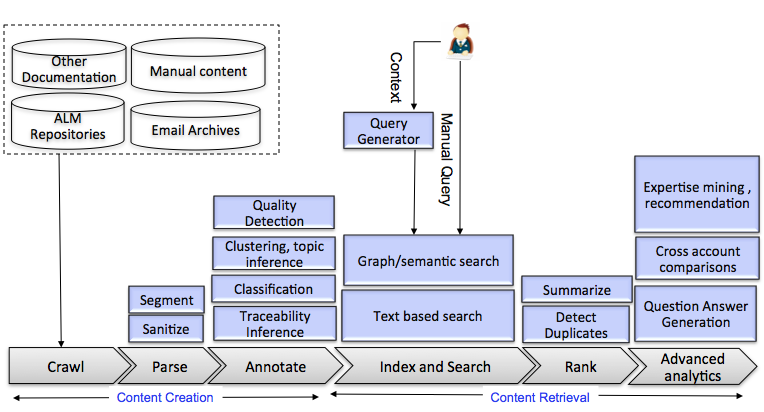
\includegraphics[scale=0.5]{figs/km.png}
	\caption{System architecture for a OKMS system for services organization.}
	\label{fig-km}
\end{figure*}


\subsection{Research Areas}

We encountered the above OKMS needs in IBM services division and made an attempt at building systems that addressed these needs. \cite{} describes a system that is in use in IBM that enables cross-account sharing of knowledge in problem tickets. \cite{} discusses the system that was built to promote solution reuse in design-build engagements centered around business process transformation. We now outline some core problems that need to be addressed to create OKMS systems in services organizations. At the simplest level, a OKMS system is a database where content can be put and retrieved. However, what content should be put, how easily can it be put and further the ease with which relevant content can be retrieved determines whether the knowledge management system would be used or not. 
Figure ~\ref{fig-km} shows the advanced the architecture for an OKMS system in services. The blue boxes indicate areas that could benefit from further research. 

\subsubsection{Content Creation}

The first challenge in building an OKMS system is identifying what data should be put in the repository and how to obtain the data. An organization has the option of mandating that each of it's employees contributes their learnings to the OKMS system. Some examples of manual knowledge creations are: (1) frequently asked question, where employee outlines the typical solutions to some common problem tickets they have resolved (2) postmortem reports, usage stories, experience reports\cite{}, that project members can create after they solve a key issue in the project. To enable solution reuse, services organizations often invest in creating software product families \cite{}. However, here it's pre-anticipated what could be some solutions that could be of interest to multiple clients in a particular domain such as healthcare and then those solutions are created with appropriate points for variability built in, so solution can be customized for any client intending to use it.  Once a project is completed, employees are also encouraged to identify reusable components in software they created and share them in the knowledge base. This approach of manual content creation adds extra burden on the employees. An open research challenge is to motivate employees to contribute high quality content in the knowledge base \cite{}. Open source forums such as stack exchange have experimented with elaborate incentive mechanisms in forms of badges to ensure questions and answer contributions on their forums \cite{}. In services organizations are reputation building incentives enough or incentives should translate to monetory benefits and/or career progression? 

Another approach for content creation is to auto-harvest artifacts produced in the SDLC lifecycle and put these in the knowledge management system. Complete traceability from requirement through code to test cases, along with their content is extractable from Application Lifecycle Management tools and this can act as solution packs to put in the repository. Similarly for ticket resolution, information about problem ticket and it's resolution is extractable from ticket management systems. Account teams periodically report on various important metrics on the applications being maintained in the client landscape such as ticket volumes, code changes, service improvement actions taken. These reports can be auto pushed into the knowledge repository. The main challenge here is crawling and parsing of this data from various tools and work product templates being used across clients and collating this information into a standardized format that can be pushed into the knowledge repository. Many of this work products are documents in proprietery formats such as Microsoft word, power point slides, visio diagrams, excel sheets. How to automate content extraction from client specific work products into the standard format used by knowledge repository is again a direction for research. One approach is to write model to model transforms where a project admin can specify the mapping \cite{}. Another challenge is that requisite traceability information that is required to understand complete context of how and why an artifact was produced, might be missing. This is because tools being used to create different SDLC artifacts have not ben integrated. In such cases, research can help come up with various heuristics to infer traceablity \cite{}. For example, if making a code commit, the developer puts in a comment like "Fixed Bug \#145", then with high confidence the change is to fix "Bug \#145" and corresponding edge between code file and bug report can be created. In text mining literature, given pieces of text the process to resolve entities and detect relationships therein is called entity resolution \cite{}. Entity resolutions techniques customized for SDLC data can help alleviate challenges in standardizing auto-harvested content.

The content put in the OKMS should be organized in such a way that retrieval becomes easier when someone needs it. The general practice is to classify OKMS content against pre-defined taxonomies. One taxonomy is obviously the object type i.e. requirement, code, problem ticket (further segmented into problem description, resolution). Another taxonomy captures the domain the artifact was produced in i.e. industry type and process area e.g. \cite{}. Another taxonomy is the technology used. Organizations spend effort building and maintaining these taxonomies. For every data that is put into the knowledge base, the content needs to be manually categorized against these pre-defined taxonomies. Classification (machine learning) based approaches can be used to auto-categorize content to these pre-defined taxonomies. These techniques rely on the availability of equal proportion of positive and negative samples to train a learning model. However, due to unavailability of training data and/or lack of differentiating features, usual learning techniques such as naive bayes, support vector machines, decision trees, might end up not giving desired efficacy (measured as precision and recall). There is need to customize more advanced learning approaches such as adaptive learning, ensemble techniques or develop new techniques that work well with SDLC data. Another interesting area for research is to explore how to help grow the taxonomy over time based on content coming in the knowledge base. Techniques such as text clustering, topic modeling \cite{} help group together similar looking content and infer topics out of them. 

The content in a OKMS database comes from various client projects. There are strict privacy constraints around what data is client confidential and hence cannot be shared. Within a single artifact itself, there might be small portions of content that are client confidential. E.g. a problem ticket might content the contact information of the user who encountered the information. How to remove client confidential data from artifacts put in the repository, how to anonimize the content so as to not disclose client identity and how to ensure that only authorized users and roles have access.

Once an OKMS system is implemented in an organization, irrespective of the approach to collect content i.e. manual, automated harvesting or hybrid, the repository starts filling up fast. Over a period of one year, the problem ticket repository we setup within IBM collected 750K tickets. Similarly, the business process solution repository has 16000 solutions. However, not all content being put in the repository is high quality and reusable. Hence, it is becomes imperative to be able to filter out useless content. One way to achieve this is by making a human vet every content being pushed in the repository and only content that is deemed high quality is published. Another approach is to ask people who are retrieving and potentially using the content, give feedback on whether they found content useful or not. The third approach that makes for an interesting research direction is to explore how a an automatic quality score can be assiged to each artifact based on content in the artifact, prior reputation of people who authored the content, whether the project was a success or not and so on. In our problem ticket repository, we experimented with calculating a quality score per ticket based on technical versus non-technical content present in the ticket \cite{}.

To summarize, content creation in OKMS provides multiple oppurtunities where research can contribute. These include: what and how to extract content from SDLC repositories and proprietry document formats, how to infer traceability between different artifacts, how to classify and categorize content, how to maintain privacy, estimate quality and motivate employees to contribute high quality content. 

\subsubsection{Content Retrieval}

A good OKMS system is one that not only had good content, but one that makes it easy to retrieve the content when needed. Typical ways to retrieve content from a knowledge base are: (1) keyword based search where user specifies a couple of words (s)he is looking for and all artifacts in the repository that contain the words from user query are returned, (2) faceted (or navigational) search where user is shown a hierarchy structure (taxonomy) and can browse information by choosing one or more values from each of the pre-defined categories. Various information retrieval models such as vector space models \cite{}, probablistic models \cite{}, latent semantic index \cite{} exist that can be used here. But inspite of easy to use search technologies being available, prior studies report that knowledge retrieval from organization wide repositories remains a challenge. As per \cite{}, while employees spend 15\% to 35\% of their time searching for information in an enterprise, they are successful less than 50\% of the time \cite{} in finding what they are looking for. 

Non-availability of content or poorly organized content can be one reason for this. Another reason could be the inadequacy of the query itself that are used to retrive the content. Suppose a user is trying to find problem tickets that resolved similar issues to what (s)he has been assigned. (S)he would pick up a couple of words from the ticket that describe the problem and use it to query the knowledge base. However, these words might not be discriminative enough and user might end up getting too many or too little search hits. Another approach could be to use complete content in the ticket and use it as query. However in this case, the search engine might end up returning irrelevant results as equal weightage was given to all words in the problem ticket. \cite{} tries to address this issue by giving more weightage to those words in the query that belong to ticket title. \cite{} parses out different datatypes from a problem ticket such as description, application information, stack trace and using a different query/search mechanism for each. E.g. instead of just specifying "null pointer exception", the query generated from a problem ticket could be---description: contains following bag of words \{null, pointer, exception\}, process: is equal to "order to cash", stack trace: contains foo.*bar. The results obtained from such a query are likely to be more precise than what a keyword search would yield. A challenge with this approach is how to compose the various clauses in the query---are they "anded" or "ored" or a combination. Another challenge is how much weightage to give to each clause when ranking the search results. \cite{} has proposed an approach called "correspondence analysis" to handle this. Recently, contextual search \cite{} has been gaining momentum. Contextual search tries to better capture a user's information need by augmenting the query with contextual information extracted from search context. It would be an interesting direction for future research to see for each of the knowledge needs in services organizations, what can make up the context, how to use this context to create the query and how to weigh different clauses in the query. 

Any search based system would return multiple results. For the user it becomes a chore in itself to go over each of the search results and identify if it is relevant or not. Techniques that can help the user easily comprehend the relevance of the returned results are much needed. Text based search engines highlight the matching words between query and content of the artifact returned. However, when the query becomes complex (as above), keyword highlighting is not of much help. In text processing domain, summarization is one approach that is used to help end users get a quick idea of what the content is about. In \cite{} authors present different techniques to summarize bug reports. Research can help in developing summarization techniques that work for other SDLC artifact such as code, requirements, solution design documents and so on. Further, out of the search results returned many artifacts could be duplicates or near duplicates of each other. In order to reduce information overload for end user, the OKMS system should be able to group together duplicates and near duplicates and be able to highlight the variances in seemingly similar artifacts returned in the search results. Duplicate bug report detection \cite{} has been a widely researched topic. Similarly for each of the artifact of interest from a services OKMS perspective, a customized duplicate detection approach might be needed. 

Most existing OKMS systems use text based IR models to store and retrieve knowledge. However, as we saw in content creation section, the repository is not just a collection of artifacts but a network of linked artifacts. Graph based search \cite{}, semantic search \cite{} are other techniques to store and retrieve knowledge and it is definitely worth investigating if any of these work better than more prevelant IR techniques for the various OKMS needs in a services organization. 

OKMS today stops at providing search capabilities. Given a user query, the system returns back matching artifacts but makes no attempt at making any deductions. Consider the scenario of troubleshooting. A user is searching through the past resolved ticket repository to see if similar issues were resolved. There are multiple reasons why the issues could have arisen. Based on past tickets, the user needs to come up with potential hypothesis of why the issue could be arising and based on conditions (s)he is seeing in the current landscape decide what hypothesis is applicable and then pick the appropriate solution. From such a user's perspective the OKMS system would be more effective if it were able to auto-generate these potential root causes and solutions hypothesis. Consider the service improvement use case, the accout team needs support from OKMS to identify similar projects, then compare the problems seen in the current project with different kind of issues arising in similar projects, then judge whether current team is doing better or worse and then decide to take some action. What kind of capabilities are needed in OKMS system to be useful in above scenarios is another area for research. 

Till now what we have discussed is what is called codification strategy \cite{} in knowledge management literature. In codification knowledge is carefully captured and stored in the database, where it can be accessed and used by anyone in the company. This strategy allows many people to search for and retrieve knowledge without having to contact the person who originally developed it. This opens up the possibility of achieving required scale in knowledge reuse in services organizations. Another strategy for knowledge management is personalization. Here knowledge is  tied to person who developed is and is shared mainly through direct person-to-person contacts. The chief purpose of knowledge management system here is to help people find and connect to other people who have requisite knowledge, not to store it. This strategy works well when knowledge cannot be codified especially knowledge required to handle situations that require complex decision making. Projects like expertise browser \cite{}, expertise recommender \cite{} have attempted to identify experts on various topics within a project. In an organization setting, what information to use to mine expertise and how to match your current context and job profile to suggest people you should have in your network is another scenario where research can help. 

To summarize, content retrieval in OKMS system provides open research problems in query generation and use of context to augment queries, search result summarization, duplicate detection, use of semantic search to improve search relevance. Further the retrieval capabilities need to move beyond just search to provide capabilities such as question-answer generation, cross-account comparison/benchmarking and expertise mining and expert recommendation.

